\newpage
\section{Konzeptfindung}

Das Endziel ist ein möglichst einfaches und zuverlässiges Gesamtkonzept, welches möglichst robust und Fehler-unanfällig funktioniert. Dies möchten wir erreichen, in dem wir vorgängig alle Lösungsansätze aus der Technologierecherche, welche mit grossen Risiken verbunden sind, erkennen und ausscheiden. Mit den verbleibenden Ansätzen wird ein Morphologischer-Kasten erstellt, um ein Gesamtkonzept zu entwickeln. Um mit dem Morphologischen Kasten die optimale Variante zu finden, wird zu einigen Teilfunktionen des Fahrzeuges eine Nutzwertanalyse erstellt.

\subsection{Vorauswahl}
    \subsubsection{Fortbewegung}
        Da das Fahrzeug in der Lage sein muss, sich an Ort und Stelle um die eigene Achse zu wenden, sind die Optionen Knicklenkung, Achsschenkellenkung und Drehschemellenkung nicht geeignet.
        Das Prinzip 'Fahrzeug ab bocken und drehen' ist als alleiniges Lenksystem ungeeignet, weil es zu viel Zeit benötigt für das Lenkmanöver. Es wird als optionalen Plan-B beibehalten für den Fall, dass das Fahrzeug beim Wenden während dem Hindernishandling verrutscht. Falls dieses Problem beim Testen auftritt, kann das System nachgerüstet werden.
    \newpage
    \subsubsection{Hindernis Bewältigung}
        \paragraph{Aufnahme}
            Da das Konzept möglichst einfach und zuverlässig gestaltet werden soll, scheiden die Ideen 'Gabelstapler' und 'Vakuumgreifer' aus der Vorauswahl aus. Der Gabelstapler erfordert eine äusserst präzise und aufwendige Sensorik, um die Löcher für die Aufnahme genau zu treffen. Der Vakuumgreifer wiederum zeigt im Vergleich zu den 'Klemmen' eine geringere Zuverlässigkeit. Um eine vergleichbare Zuverlässigkeit zu erreichen, wären umfangreiche Tests erforderlich, ohne dass der Vakuumgreifer dabei signifikante Vorteile gegenüber den 'Klemmen' bieten würde.

        \subparagraph{Nutzwertanalyse Aufnahme}
        Damit eine genauere Analyse zwischen Klemme Breitenweg und Klemme Längsweg durchgeführt werden konnte, wurde eine Nutzwertanalyse durchgeführt. Der Gewinner war Klemme Breitenweg, was auch in Tabelle \ref{tab:konzept_nutzwertanalyse_aufnahme} ersichtlich ist.
        
        \begin{table}[H]
        \resizebox{\textwidth}{!}{
         \centering
         \renewcommand{\arraystretch}{1.5}
             \begin{tabular}{|c|>{\raggedright} p{3cm}|c|c|c|>{\raggedright} p{3cm}|c|c|>{\raggedright\arraybackslash}p{3cm}|}
                \hline
                \multicolumn{3}{|c|}{} & \multicolumn{3}{c|}{\textbf{Klemme Breitenweg}} & \multicolumn{3}{c|}{\textbf{Klemme Längsweg}} \\ \hline
                \textbf{Kriterium} & \textbf{Erklärung} & \textbf{Gewichtung} & \textbf{Bewertung} & \textbf{Punkte} & \textbf{Begründung} & \textbf{Bewertung} & \textbf{Punkte} & \textbf{Begründung} \\ \hline
                Sicherer Halt & Wie gut hält das Hindernis in der Halterung & 35 & 7 & 245 & Relativ starke Punktlast, aber dennoch sehr guter Halt & 8 & 280 & Große Fläche zur Kraftübertragung, stabil und sehr guter Halt \\ \hline
                Präzision & Wie präzise ist die Vorrichtung, auch wenn das Fahrzeug nicht genau zentriert vor dem Hindernis steht & 30 & 7 & 210 & Siehe Kapitel Präzision, detaillierte Erklärung & 4 & 120 & Siehe Kapitel Präzision, detaillierte Erklärung \\ \hline
                Komplexität & Wie aufwendig ist die Konstruktion & 20 & 5 & 100 & Nicht sehr komplex & 5 & 100 & Nicht sehr komplex \\ \hline
                Kosten & Wie viel kostet die Vorrichtung & 15 & 4 & 60 & 3D-Druck möglich & 4 & 60 & 3D-Druck möglich \\ \hline
                \multicolumn{2}{|r|}{\textbf{Nutzwert:}} & 100 & & 615 & & & 560 & \\ \hline
            \end{tabular}
         }
            \caption{Nutzwertanalyse der Klemmen Breitenweg und Längsweg, Der gewinner ist Klemme Breitenweg}
            \label{tab:konzept_nutzwertanalyse_aufnahme}
        \end{table}

        \newpage
            
            \subparagraph{Präzision}

            In der Nutzwertanalyse wird erwähnt, dass das Kriterium Präzision eine genauere Erklärung benötigt. Die Präzision der Klemme Breitenweg kann besser erreicht werden als bei der Klemme Längsweg. Einerseits kann, wie in den Abbildungen \ref{img:konzept_zentrierung_1} und \ref{img:konzept_zentrierung_2} gezeigt, eine Zentrierung bei der Klemme Breitenweg eingebaut werden. Diese Zentrierung fehlt bei der Klemme Längsweg. Da unter anderem das Ziel ist, das Hindernis möglichst zentriert wieder auf dem Klebeband abzustellen, verliert hier die Klemme Längsweg an Punkten. In Abbildung \ref{img:konzept_zentrierung_3} wird dargestellt, dass, wenn das Fahrzeug nicht perfekt mittig auf das Hindernis zufährt, automatisch ein Fehler generiert wird, weil das 'Offset' nicht, ohne komplexere Sensorik, miteinbezogen werden kann.


            \begin{figure}[h!]
                \centering
                \begin{minipage}{0.48\textwidth}
                    \centering
                    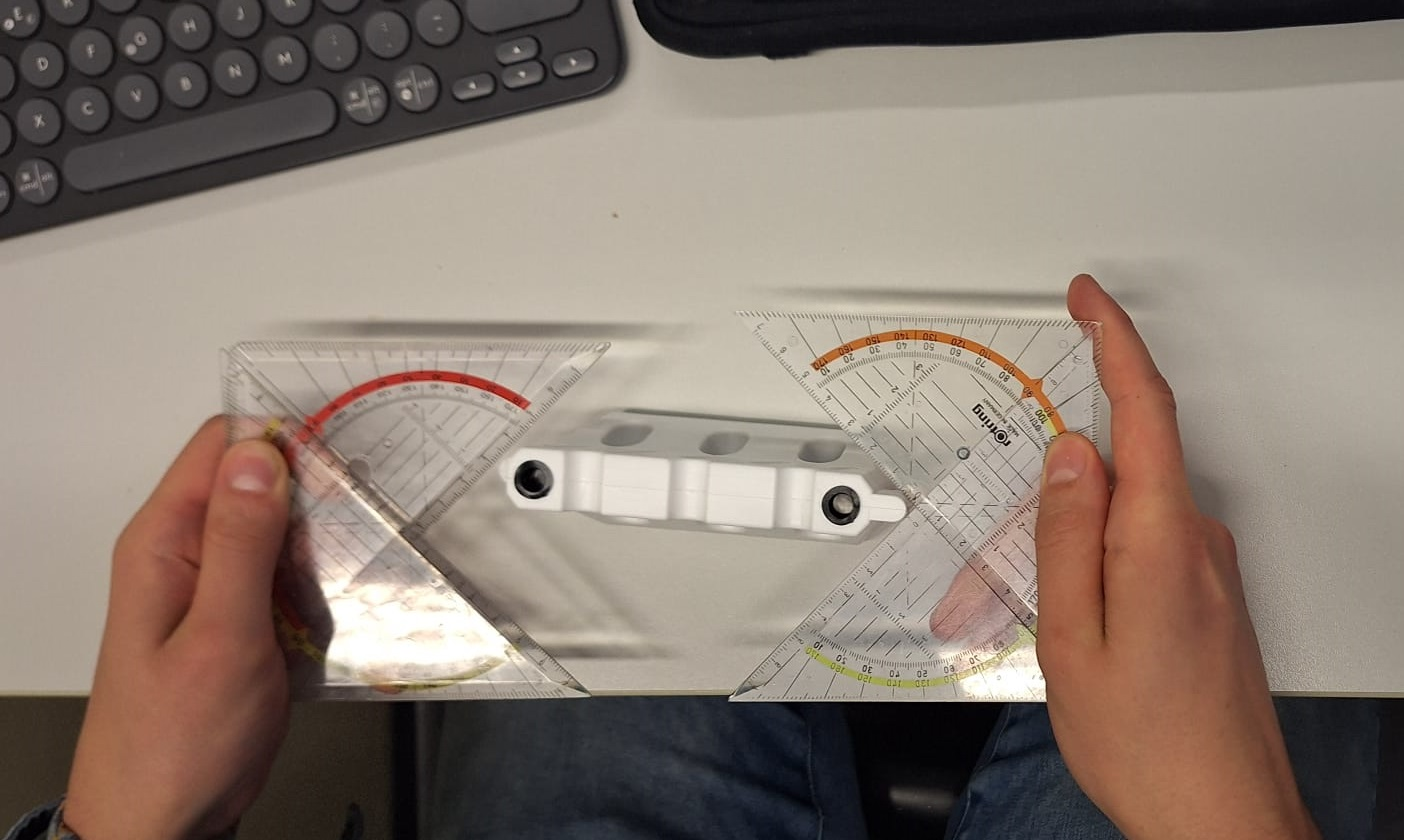
\includegraphics[width=\linewidth]{img/konzeptfindung/klemme_breitenweg_zentrierung_1.jpeg}
                    \caption{Darstellung Zentrierung bei Klemme Breitenweg - Bild 1}
                    \label{img:konzept_zentrierung_1}
                \end{minipage}
                \hfill
                \begin{minipage}{0.48\textwidth}
                    \centering
                    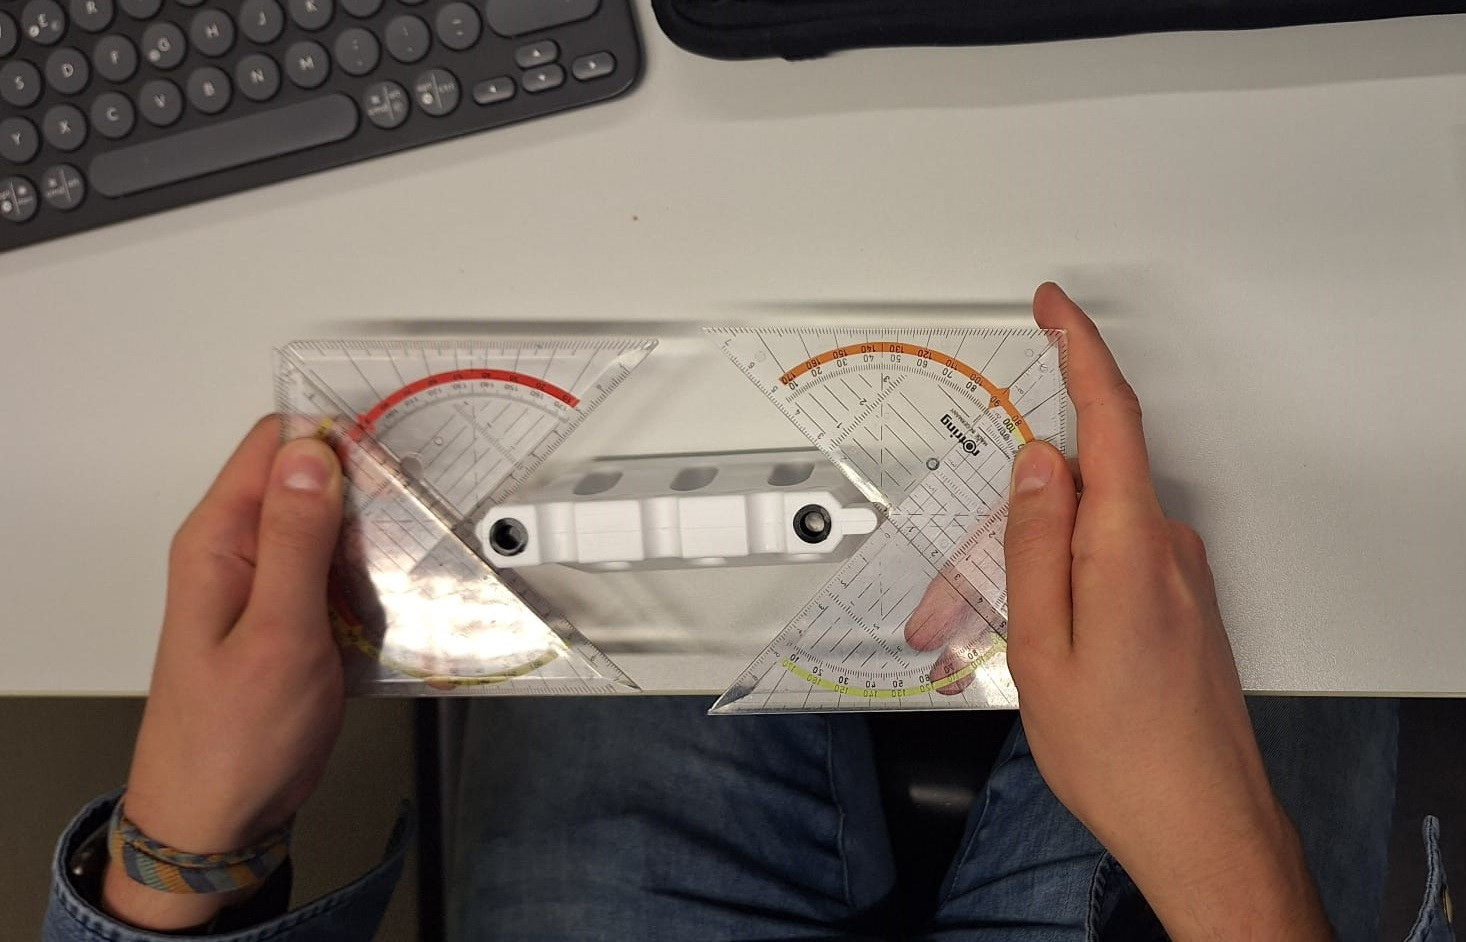
\includegraphics[width=\linewidth]{img/konzeptfindung/klemme_breitenweg_zentrierung_2.jpeg}
                    \caption{Darstellung Zentrierung bei Klemme Breitenweg - Bild 2}
                    \label{img:konzept_zentrierung_2}
                \end{minipage}
                \caption{Vergleich der Zentrierung bei Klemme Breitenweg}
            \end{figure}


        \begin{figure}[h!]
            \centering
            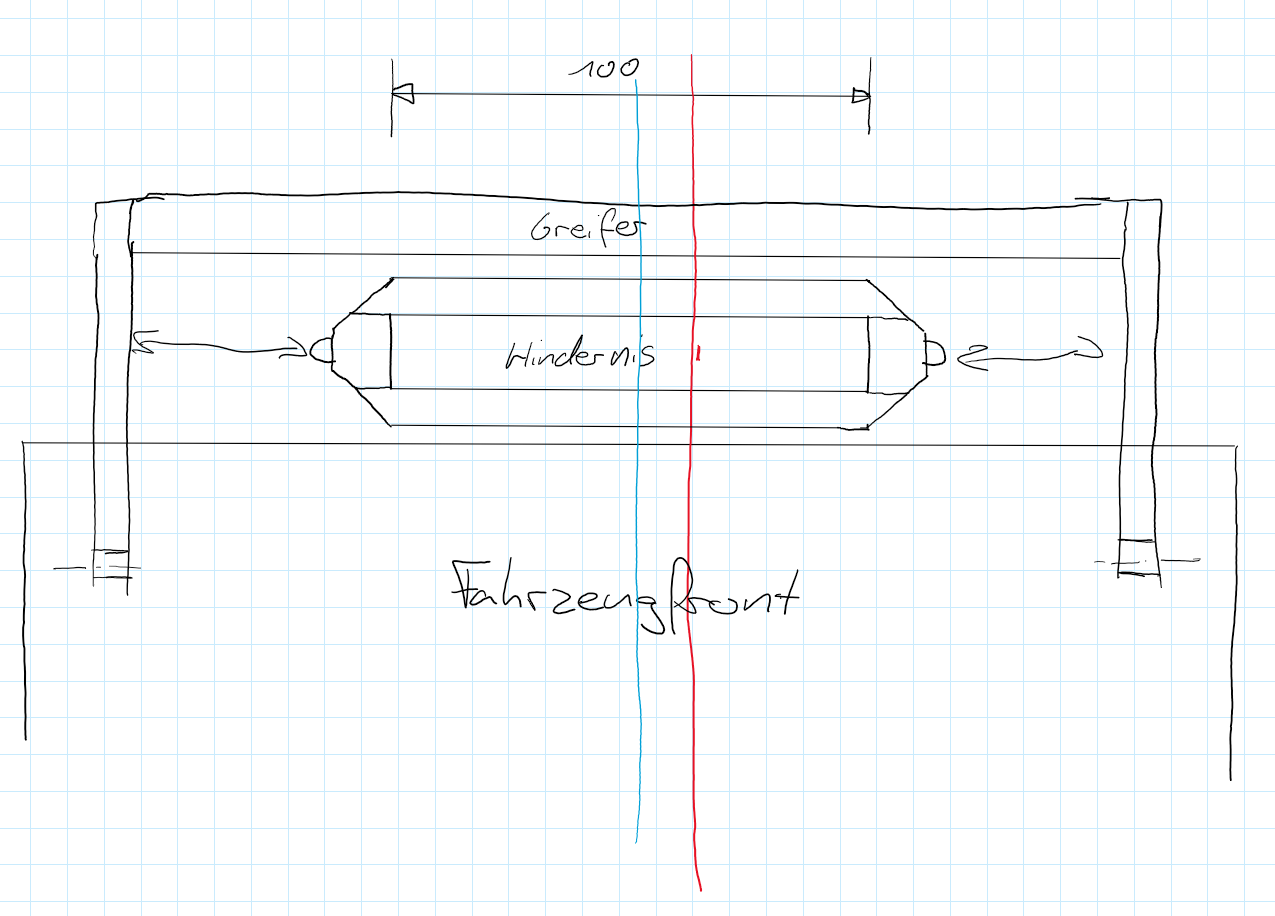
\includegraphics[width=0.48\textwidth]{img/konzeptfindung/Klemme_Langsweg_off_center.png}
            \caption{Darstellung 'Offset' bei Klemme Längsweg}
        \label{img:konzept_zentrierung_3}
        \end{figure}  
                        
        \newpage         
        \paragraph{Rotation und Translation}
        Da ein beweglicher Arm die Komplexität nicht nur mechanisch, sondern auch in den Bereichen Sensorik und Software erheblich erhöht, wird diese Option aus der Vorauswahl ausgeschlossen. Die Einführung eines Arms fügt zusätzliche Komplexität hinzu, ohne die Möglichkeit, in anderen Bereichen Vereinfachungen zu erzielen. Dies widerspricht unserer Grundidee, eine möglichst einfache und zuverlässige Lösung zu entwickeln.

\subsubsection{Elektrotechnik}
    \paragraph{}

\subsection{Objekterkennung}



\subsubsection{Simulator}
    \paragraph{}

\subsection{Morphologischer Kasten}
        